\chapter{Traffic Shaping in Userspace}
\label{cap:userspace}
Come speigato nel capitolo precedente, l'uso del comando \texttt{tc} in ambienti containerizzati come Kathará 
presenta limiti legati alla disponibilità di moduli all'interno del kernel dell'host. \\ 
Per garantire portabilità e riproducibilità indipendentemente dal sistema di esecuzione è necessario cambiare approccio, 
spostando la logica di shaping all'interno dello userspace.

\begin{intuition}[Prelevare i pacchetti dal Kernel]
  Una soluzione per spostare lo shaping in user space potrebbe essere quella selezionare correttamente e fermare momentaneamnte i pacchetti nel kernel,
  permettendo a un processo in user space di decidere quanto e se trattenerli.
\end{intuition}
Questa modalità, però, richiede di intercettare specifici pacchetti,
bloccarli per un determinato tempo e avere un processo capace di decidere quali scartare e quali rallentare.

\section{Iptables}
Il primo punto da chiarire è come selezionare i pacchetti corretti su cui effettuare lo shaping.
Nel kernel Linux questo è possibile farlo tramite il framework \textbf{Netfilter}, che implementa lo strumento \textbf{Iptables} in user space \cite{netfilter}.

\begin{defn}[Iptables]
  Netfilter mette a disposizione una serie di \textbf{hooks}, in cui possono essere associate delle regole per definire i criteri per scartare, accettare o inoltrare un pacchetto. \\
  \texttt{iptables} è il comando in user space che permette di creare queste regole, raccogliendole in \textbf{catene}.
  Le catene, a loro volta, vengono inserite all'interno di specifiche \textbf{tabelle} \cite{iptables}.
\end{defn}
Esistono diverse catena disponibili di base:
\begin{itemize}
  \item \textbf{PREROUTING:} intercetta tutti i pacchetti in ingresso nell'interfaccia di rete, prima che venga effettuato il routing.
  \item \textbf{INPUT:} gestisce i pacchetti destinati ai processi in esecuzione sul'host.
  \item \textbf{FORWARD:} intercetta i pacchetti che l'host deve instradare verso un'altra destinazione.
  \item \textbf{OUTPUT:} gestisce i pacchetti che i processi in esecuzione sul'host devono inviare sulla rete.
  \item \textbf{POSTROUTING:} intercetta i pacchetti in uscita dopo che è stato effettuata la decisione di instradamento.
\end{itemize}
Ma anche diverse tabelle indipendentementi possibili:
\begin{itemize}
  \item \textbf{Filter:} tabella di dafault. Usata per le regole di filtraggio sui pacchetti.
  \item \textbf{Nat:} tabella con le regole di NAT.
  \item \textbf{Mangle:} usata per modificare parti dei pacchetti.
  \item \textbf{Raw:} assegna un mark ai pacchetti, per non essere gestiti dal sistema tracciamento dello stato delle connessione (\textbf{conntrack)}.
    Questa tabella ha priorità più alta e viene chiamata prima delle altre.
\end{itemize}
La combinazione della tabella \textbf{Raw}, visto l'elevata priorità che gli viene assegnata, con la catena \textbf{OUTPUT} che permette di prendere i pacchetti
prodotti da un processo in esecuzione nell'host, ci permette di risolvere la prima parte dell'intuizione di inzio capitolo \ref{cap:userspace}:
selezionare i pacchetti corretti per lo shaping, specificando, nel caso, porte, protocolli o altre caratteristiche con il comando \texttt{iptables}.

\begin{figure}[!htb]
    \centering
    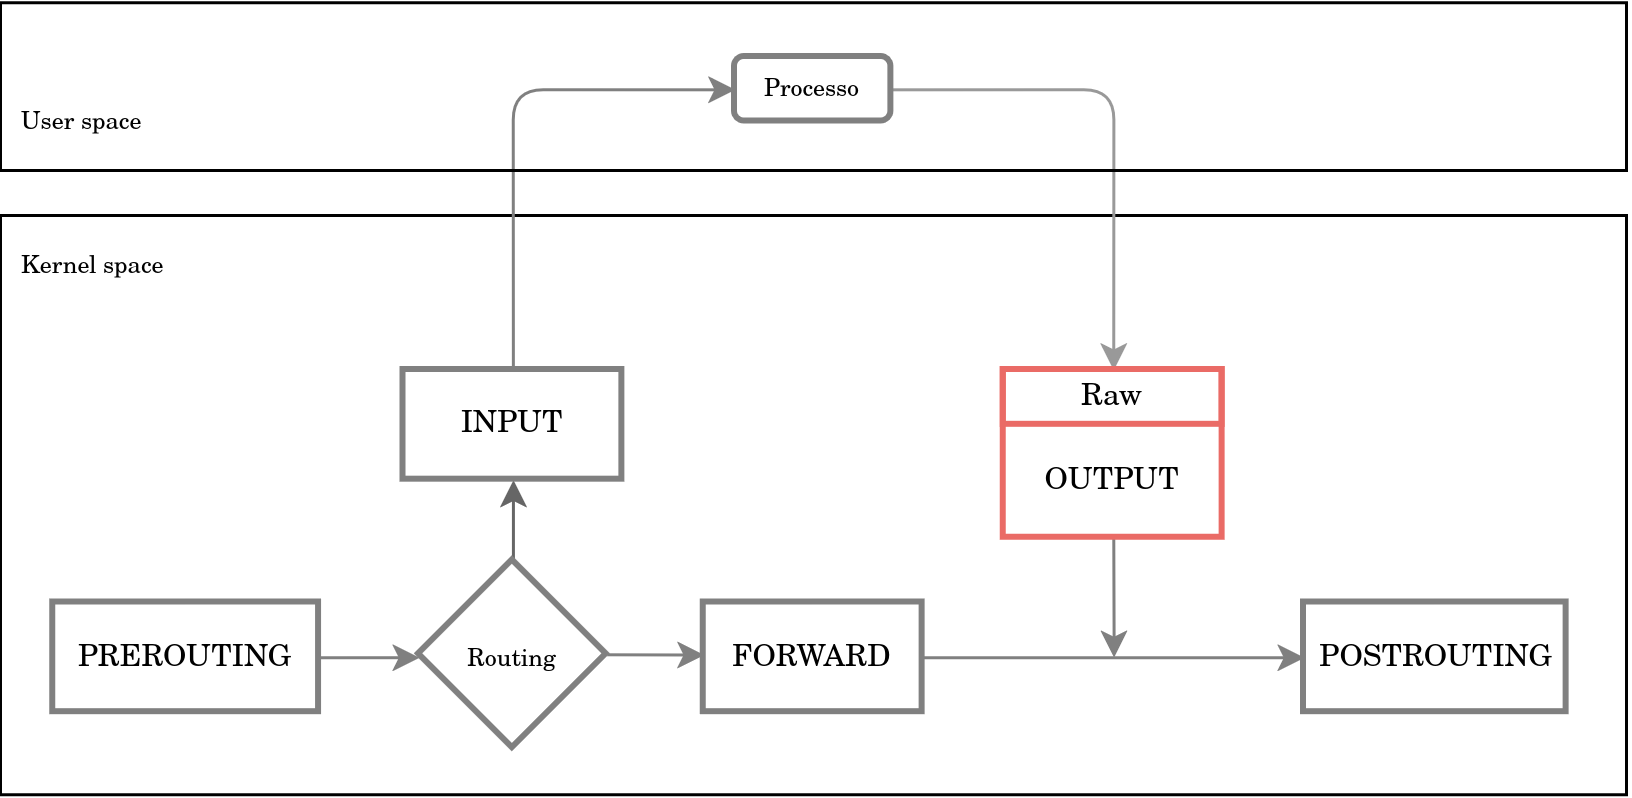
\includegraphics[width=0.8\linewidth]{Images/damper/iptables.png}
    \caption{Rappresentazione della situazione descritta.}
\end{figure}

\subsection{Target NFQUEUE}
Avendo selezionato i pacchetti corretti, è necessario capire come poterli trattenere nel kernel, per metterli a disposizione del processo in user space. \\ 
La soluzione è nelle azioni o \textbf{target}, messe a disposizione da Netfilter \cite{netfilter}, che normalmente vengono usate quando una regola trova corrispondenza:
\begin{enumerate}
  \item \textbf{ACCEPT:} accetta il pacchetto.
  \item \textbf{DROP:} scarta il pacchetto.
  \item \textbf{RETURN:} interrompe la catena corrente.
  \item \textbf{NFQUEUE:} accoda il pacchetto in una coda numerata nel kernel.
\end{enumerate}
Il target \textbf{NFQUEUE} fa esattamente quello che serve nella soluzione proposta a inizio capitolo. \\
\vspace*{0.01\textheight}
Nello specifico, si hanno diverse fasi:
\begin{enumerate}
  \item Il pacchetto viene selezionato tramite il comando \texttt{iptables}, specificando i criteri che servono.
  \item Il target NFQUEUE permette di spostarlo in una coda all'interno del kernel.
  \item Il kernel, tramite \textbf{netlink} \cite{netlink}, crea un messaggio con i dati del pacchetto che servono al processo in userspace e lo invia tramite socket.
  \item Il processo in userspace, tramite la libreria \textbf{libnetfilter\_queue} \cite{libnetfilter-queue}, riceve il messaggio e decide come gestire il pacchetto, 
    potendo anche ritardare la decisione, effettuando di conseguenza un'azione di shaping.
\end{enumerate}

\newpage
\subsection{Netlink}
\begin{defn}[Netlink]
  Netlink è un protocollo utilizzato per far comunicare processi in kernel space con processi in userspace.
\end{defn}
Mette a disposizione un interfaccia socket che comunica con una API del kernel, permettedno quindi lo scambio di informazioni.
Esistono diversi tipi di \textbf{famiglie}, che permettono di scegliere con che gruppo comunicare. Per le NFQUEUE esiste \texttt{NETLINK\_QUEUE} \cite{netlink}.

\subsection{Libnetfilter\_queue}
\begin{defn}[libnetfilter\_queue]
  Libreria in userspace che tramite una API permette di interagire con i pacchetti fermati in una coda nel kernel \cite{libnetfilter-queue}.
\end{defn}
Sfrutta il protoccolo Netlink per comunicare con il kernel, permette al processo in userspace di fare diverse azioni:
\begin{enumerate}
  \item \textbf{Accept:} fa passare il pacchetto alle regole e catene successive.
  \item \textbf{Drop:} fa scartare il pacchetto.
  \item Alterare il contenuto del pacchetto.
\end{enumerate}
Funzionando in maniera asincrona, può mandare la decisione in un qualsiasi momento, visto che richiede solo l'id del pacchetto. 
Questo è il dettaglio che permette al processo di effetuare lo shaping.

\begin{figure}[!htb]
    \centering
    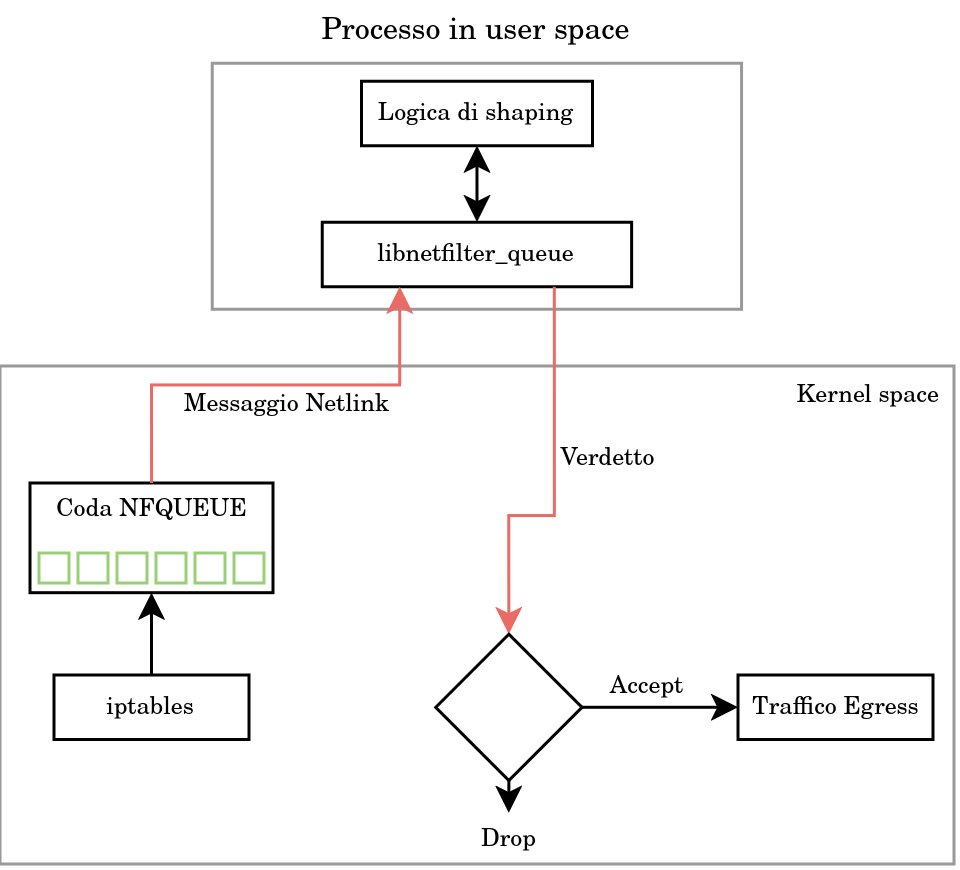
\includegraphics[width=0.8\linewidth]{Images/damper/nfqueue.png}
    \caption{Ciclo di vita pacchetto NFQUEUE.}
\end{figure}
L'ultimo pezzo mancante è il programma in user space che implementi tutta la logica di shaping vista nel capitolo \ref{cap:tc}.

\section{Damper}
\begin{defn}[Damper]
  Damper \cite{damper} è programma open-source scritto in linguaggio \textbf{C}, che tramite la libreria \texttt{<libnetfilter\_queue.h>} messa a disposizione da Netfilter \cite{netfilter},
  permette di interagire con i pacchetti nella coda NFQUEUE nel kernel.
\end{defn}
Implementa, tramite un file di configurazione, una logica di shaping simile a un algortimo \textbf{leaky bucket}, dove però latenza dipende dalla dimensione del pacchetto.

\begin{defn}[Leaky Bucket]
  A differnza dell'algoritmo token bucket, che accumola gettoni all'interno di un contenitore e invia pacchetti solo se si hanno abbastanza gettoni, 
  l'algoritmo leaky bucket usa un approccio diverso: il bucket raccoglie tutti i pacchetti e li invia a una velocità costante, non vengono usati token.
\end{defn}

\subsection{Logica di funzionamento}
La configurazione dei parametri per il traffic shaping viene fornita tramite il file \texttt{damper.conf}. 
All'interno del programma la funzione \texttt{read\_config()} si occupa di fare il parsing del file e di salvare tutte le informazioni nella struttura dati \texttt{struct userdata}.

\begin{figure}[!htb]
    \centering
    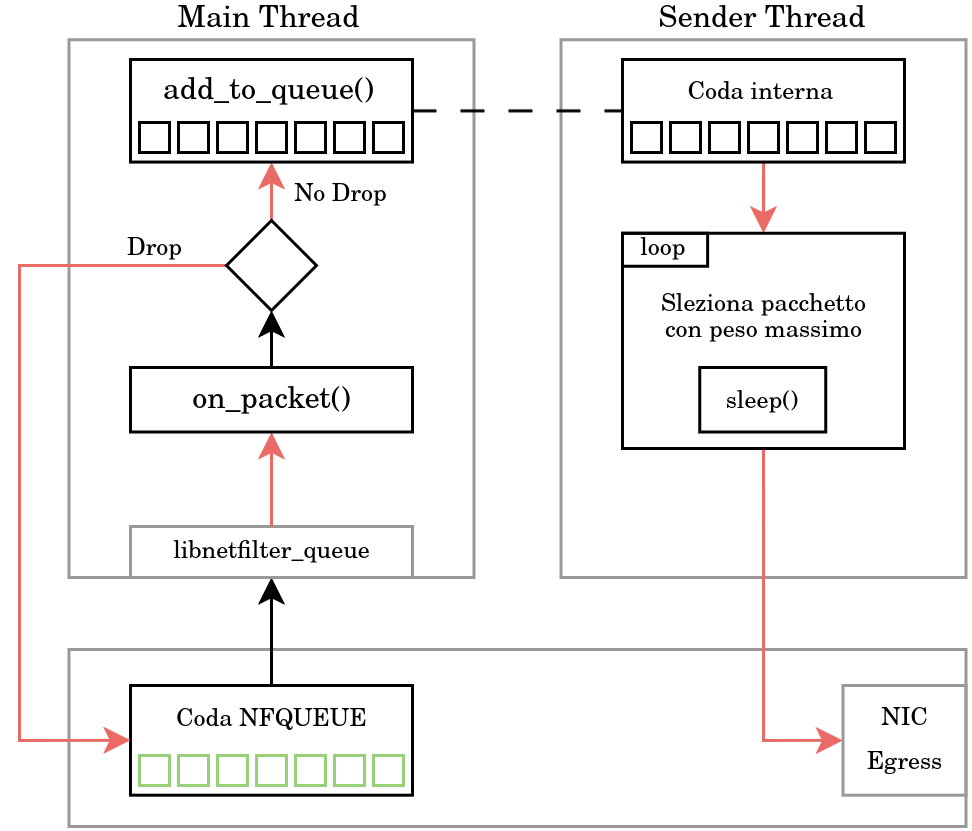
\includegraphics[width=0.8\linewidth]{Images/damper/damper.png}
    \caption{Funzionamento di Damper.}
\end{figure}

La logica principale è divisa in due thread: il \textbf{main thread} e il \textbf{sender thread}. \\
Il primo, è il thread che tramite le funzioni fornite dalla libreria \texttt{<libnetfilter\_queue>} gestisce i pacchetti della NFQUEUE. 
Utilizza, oltre a \texttt{read\_config()}, una serie di funzioni:
\begin{itemize}
  \item \texttt{on\_packet()}: funzione che gestisce ogni pacchetto della NFQUEUE, assegnandoli un \textbf{peso}. 
    Se negativo, viene inviato un verdetto di Drop per scartare il pacchetto, altrimenti viene invocata un'altra funzione per inserire il pacchetto in una coda.
  \item \texttt{add\_to\_queue()}: funzione che copia l'id, la dimensione e il payload del pacchetto in un array di \texttt{ struct packet},
    ossia una strttura dati usata per contenere i dati di un pacchetto della NFQUEUE in user space. Se il vettore è pieno, viene inviato un verdetto di Drop per scartare il pacchetto con il peso minore.
\end{itemize}
Il secondo thread, invece, implementa lo shaping tramite la funzione \texttt{sender\_thread()}. Ciclo continuo che, dall'array dei pacchetti, trova quello con il peso maggiore e genera un verdetto di Accept. 
Alla fine di ogni ciclo, però, viene fatta una sleep di un numero di secondi, per fare lo shaping effettivo. La formula per il calcolo del tempo è la seguente:
\[
t = \frac{(\text{packet.size} * 1000000000)}{\text{rate}}
\]
Il risultato saranno i nanosecondi che rallenteranno l'invio del verdetto.

\subsection{Configurazione}
Damper, per funzionare ha bisogno di un file di configurazione, ossia \texttt{damper.conf}. All'interno si possono configurare i diversi moduli per calcolare il peso dei pacchetti 
e inserire i parametri per la parte di traffci shaping.

\begin{damper}[damper.conf]
# nfqueue queue id
queue 3

# traffic limit in bits per second (suffixes K, M and G allowed)
limit 20M

# queue length
packets 100

# modules
# number of recent flows
inhibit_big_flows nrecent 10
# dump debug info every 5 seconds
#inhibit_big_flows debug 5

# entropy module
entropy nrecent 10
#entropy debug 5
entropy k 2.0
# you can override source or destination port for this module
#entropy sport 0
#entropy dport 0

#bymark module
#traffic with mark 101 gets weight 0.2
bymark 101 0.2
#traffic with mark 102 gets weight 0.5
bymark 102 0.5

\end{damper}
Per usarlo è possibile clonare la repository disponibile su GitHub \cite{damper}:
\begin{bash}[Clonazione]
git clone https://github.com/vmxdev/damper.git
\end{bash}
Successivamente è possibile compilarlo, installando prima l'unica dipendenza del programma: \texttt{libnetfilter\_queue}.
\begin{bash}[Compilazione]
gcc -Wall -pedantic damper.c modules.conf.c -o damper -lnetfilter_queue -pthread -lrt -lm
\end{bash}
Dopo aver ottenuto l'eseguibile \texttt{damper}, è possibile avviarlo, passando come unico parametro il file di configurazione.
\begin{bash}[Esecuzione]
./damper damper.conf
\end{bash}
Nel prossimo capitolo \ref{cap:esempi}, dove aver trovato una modalità per fare traffic shaping in user space, si dimostrerà la fattibilità e possibili limiti.
